\section{Attention and Transformers}
\begin{figure}[ht]
    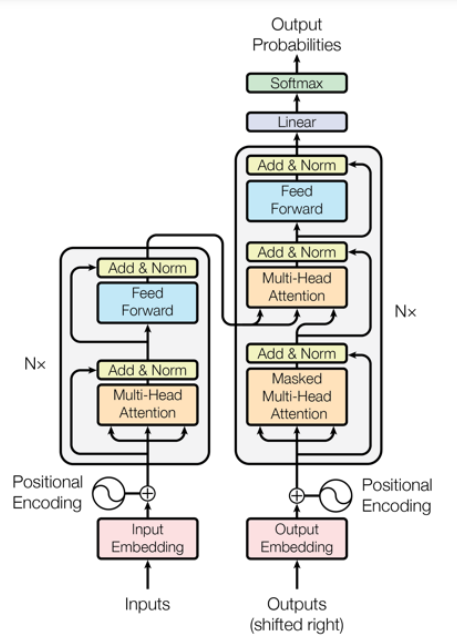
\includegraphics[width=0.6\columnwidth]{figures/AttentionTransformer/Transformer.png}
\end{figure}
\subsection{Sequence Processing}
\subsubsection{Recurrent Neural Networks (RNNs)}
\begin{itemize}
    \item Process sequences using recurrent cells with an internal state \( h \).
    \item Computation at each time step:
    \[
    h_t = \sigma(W_{hh} h_{t-1} + W_{xh} x_t + b_h)
    \]
    \item Output:
    \[
    y_t = W_{hy} h_t + b_y
    \]
    \item Common challenges: vanishing and exploding gradients.
\end{itemize}

\subsubsection{Advanced RNN Variants}
\begin{itemize}
    \item LSTMs handle long-term dependencies using gates:
    \[
    c_t = f_t \odot c_{t-1} + i_t \odot \tanh(W_c x_t + U_c h_{t-1} + b_c)
    \]
    \[
    h_t = o_t \odot \tanh(c_t)
    \]
    \item \(c_t\) long term memory
    \item \(h_t\) short term /working memory
    \item GRUs simplify LSTMs by merging the forget and input gates:
    \[
    h_t = (1 - z_t) \odot h_{t-1} + z_t \odot \tilde{h}_t
    \]
\end{itemize}
\begin{figure}
    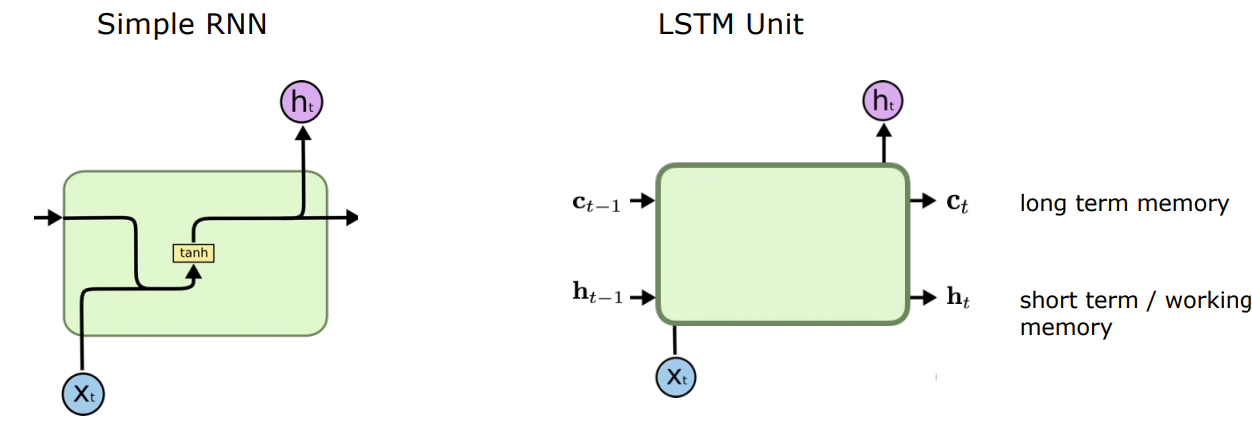
\includegraphics[width= \columnwidth]{figures/AttentionTransformer/RNNLSTM.png}
\end{figure}
\subsection{Attention Mechanism}
\subsubsection{Concept and Applications}
\begin{itemize}
    \item Attention aligns inputs with outputs for tasks like translation and image captioning.
    \item Improves handling of long sequences and offers interpretability.
\end{itemize}

\subsubsection{Attention Calculation}
\begin{itemize}
    \item Compute attention weights:
    \[
    \text{score}(q, k) = \frac{q \cdot k}{\sqrt{d_k}}
    \]
    \item Normalize weights with softmax:
    \[
    \alpha_{ij} = \frac{\exp(\text{score}(q_i, k_j))}{\sum_{j'} \exp(\text{score}(q_i, k_{j'}))}
    \]
    \item Compute the attention output as a weighted sum of values:
    \[
    \text{Attention}(Q, K, V) = \text{softmax}\left(\frac{QK^\top}{\sqrt{d_k}}\right)V
    \]
\end{itemize}

\subsection{Transformer Architecture}

\subsubsection{Encoder Architecture}
\begin{itemize}
    \item The encoder consists of \( N \) identical layers, each with:
    \begin{enumerate}
        \item Multi-head self-attention:
        \[
        \text{MultiHead}(Q, K, V) = \text{Concat}(\text{head}_1, \ldots, \text{head}_h)W^O
        \]
        where
        \[
        \text{head}_i = \text{Attention}(QW_i^Q, KW_i^K, VW_i^V)
        \]
        \item A feedforward network applied to each position:
        \[
        \text{FFN}(x) = \text{ReLU}(0, xW_1 + b_1)W_2 + b_2
        \]
        \item Residual connections and layer normalization for stability:
        \[
        \text{Output} = \text{LayerNorm}(x + \text{SubLayer}(x))
        \]
    \end{enumerate}
\end{itemize}

\subsubsection{Decoder Architecture}
\begin{itemize}
    \item The decoder mirrors the encoder but includes an additional sub-layer for cross-attention:
    \begin{enumerate}
        \item Masked multi-head self-attention:
        \[
        \text{Attention}(Q, K, V) = \text{softmax}\left(\frac{QK^\top}{\sqrt{d_k}}\right)V
        \]
        Masking prevents the decoder from seeing future tokens during training.
        \item Cross-attention, where queries come from the decoder, and keys/values come from the encoder.
        \item Feedforward network and residual connections (as in the encoder).
    \end{enumerate}
    \item A final linear layer projects the decoder's output to the vocabulary size, followed by a softmax:
    \[
    p(y_t | y_{<t}, x) = \text{softmax}(W_s h_t + b_s)
    \]
\end{itemize}

\subsubsection{Positional Encoding}
\begin{itemize}
    \item Adds sequence order information:
    \[
    PE_{\text{pos}, 2i} = \sin\left(\frac{\text{pos}}{10000^{2i/d_{\text{model}}}}\right)
    \]
    \[
    PE_{\text{pos}, 2i+1} = \cos\left(\frac{\text{pos}}{10000^{2i/d_{\text{model}}}}\right)
    \]
\end{itemize}